\documentclass{article}
\usepackage{amsmath, amsfonts, amssymb, amsthm, stmaryrd}
\usepackage{enumitem}
\usepackage{hyperref}
\usepackage{bbm}
\usepackage[ruled,linesnumbered]{algorithm2e}

\usepackage[verbose=true,letterpaper]{geometry}
\newgeometry{
  textheight=9.5in,
  textwidth=6.5in,
  top=0.5in,
  headheight=12pt,
  headsep=25pt,
  footskip=30pt
}
\setlength{\parskip}{0.5em} % blank lines between paragraphs
\usepackage{tikz}
\usepackage{pgfplots}

%%%%%% Commands and theorems
\theoremstyle{plain}
\newtheorem{Theorem}{Theorem}
\newtheorem{Proposition}{Proposition}
\newtheorem{Corollary}{Corollary}
\newtheorem{Lemma}{Lemma}

\theoremstyle{remark}
\newtheorem{Definition}{Definition}
\newtheorem{Assumption}{Assumption}
\newtheorem*{remark}{Remark}

\renewcommand{\P}{\mathbb{P}}
\newcommand{\E}{\mathbb{E}}
\newcommand{\R}{\mathbb{R}}
\newcommand{\N}{\mathbb{N}}
\renewcommand{\S}{\mathfrak{S}}

\newcommand{\sign}{\text{sign}}
\newcommand{\1}{\mathbbm{1}}
\newcommand{\id}{\mathrm{id}}

\newcommand{\argmin}{\arg\min}

\usepackage{color}
\usepackage{array}
\newcolumntype{L}[1]{>{\raggedright\let\newline\\\arraybackslash\hspace{0pt}}m{#1}}
\usepackage{todonotes}
\newcommand{\todoT}[1]{\todo[inline,color=blue!40]{{\textbf{T:}~}#1}}

\usepackage{enumitem}

% Have descriptions with italic and bullets:
\setlist[description]{font=\normalfont\itshape\textbullet\space}
% To include the section number in the equation numbering:
\numberwithin{equation}{section}

\title{Adaptive stopping in Monte-Carlo evaluation for Deep RL}
\date{}
\begin{document}
\maketitle
\section{Description of the problem}
In Reinforcement Learning, we often use Monte-Carlo methods to evaluate the performances of an algorithm. In particular, if we denote $e(A)$ some evaluation of algorithm $A$, the global score of an algorithm by
$$S(A)=\frac{1}{N}\sum_{i=1}^N e_i(A) $$
where $e_1(A), \dots,e_N(A)$ are the evaluation of the algorithm $A$ on $N$ different seeds (i.e. $e_1(A),\dots,e_N(A)$ are supposed i.i.d).

\subsection{Goal and requirements for the algorithm}

The goal of this article is, given two agents $A_1$ and $A_2$, to evaluate how high $N$ must be to be certain that either $\E[e_1(A_1)]=\E[e_2(A_2)]$ or $\E[e_1(A_1)]\neq \E[e_2(A_2)]$, i.e. do the two algorithms perform similarly or is one better than the other ? This is a trade-off between computational time and the need to assess correctly the scores of $A_1$ and $A_2$. The main properties that we want for our algorithm are as follows:

\begin{description}
\item[Multiprocessing] The algorithm should be able to treat batch of datas.
\item[Non-Parametric] The algorithm should be non-parametric.
\item[Fixed Budget] The algorithm should have a fixed maximum number of iterations used.
\item[Sample efficient] The algorithm should stop as soon as possible in practice.
\end{description}

One algorithm that verifies all the properties listed above is a group sequential permutation test that we will describe in this article.

\subsection{Alternative approaches}

\paragraph{Fully Sequential testing}
In the sequential testing setting, the data are handled one after the other, there is no batch of data. This is not adapted to our problem because in practice, one is often capable of training several agents in parallel, hence the evaluations are received by batch.

\paragraph{SPR/GLR test}
A particular class of sequential test often used are the Sequential Probability Ratio test and the Generalized Likelihood Ratio test. Both of these tests could be generalized to a group-sequential context but they both depend strongly on a parametric model for the data. However, the reward distribution of RL algorithms is often heavy-tail and multi-modal and as a consequence it is difficult to use a parametric model to represent all of them efficiently and simultaneously for several agents, each with a different reward distribution. Moreover, because we want to deal with small sample-sizes, the asymptotic of the central limit theorem is not adapted.

\paragraph{Bandits (Best arm identification or Ranking)} Our objective is close to the objective of ranking bandits algorithms. However compared to bandits we want to at the same time \textit{minimize the stopping time} (similar to fixed-confidence setting) of the algorithm and have a \textit{fixed maximum budget} (similar to fixed-budget setting). In our algorithm we allow for a type I error of $\alpha \in (0,1)$, which is very similar to the fixed confidence setting while still having a fixed budget. Then, compared to the fixed budget setting we allow a larger error rate and as a consequence we are more sample efficient than bandits algorithms.

% \subsection{Notations}
% We denote by $e(A)$ the evaluations of an algorithm $A$, $T$ is the test statistic constructed using 

\section{Description of the methods used in the algorithm}
\subsection{Group sequential testing}
\todoT{Explain why must be careful when doing GST and that we can't just do several tests. Maybe also motivate using the confidence interval approach from NIPS article.}

To choose $N$ adaptively, we propose to use group sequential testing (GST). GST are used in particular in clinical trials in which case an early stopping is desirable when comparing two drugs. We choose to use GST in particular and not sequential testing because the data are often naturally grouped due to the parallelization of the computation.

GST often suppose strong models on the data, in particular it is often supposed that the data are i.i.d. from a Gaussian distribution. This assumption is often not verified in the case of $e_i(A)$ being evaluations from a RL algorithm. In particular, the distribution of $e_i(A)$ often presents several modes and it can sometimes contain outliers.

\todoT{Explain why several modes and give examples of distributions of DeepRL algos on classical environments. Ref https://arxiv.org/pdf/1806.08295.pdf on this also.}

The presence of several modes in the distributions of the evaluations and the difficulty to make any distributional assumption justify a non-parametric approach of the problem, but to further justify this approach we did a study of the effect of model misspecification on simulated data when using Gaussian GST algorithm.


 
\subsection{High level description of the algorithm for two agents}
In the case where only two agents are compared, we use the following algorithm (see Section~\ref{sec:multi} for the multi-agent and fully developped version of the algorithm).

\begin{algorithm}[h]
\SetAlgoLined
\SetKwInput{KwParameter}{Parameters}
\KwParameter{Agents $A_1,A_2$, environment $\mathcal{E}$, number of blocks $K \in \N^*$, size of a block $N$, level of the test $\alpha\in (0,1)$.}
Define $2NK$ different seeds $s_{1,1},\dots,s_{1,N},s_{2,1},\dots,s_{2,N}$.\\
\For{$k=1,\dots,K$}{
\For{$i=1,2$}{
Train agent $A_i$ on environment $\mathcal{E}$ with the seeds $s_{i,kN},\dots,s_{i,(k+1)N}$.\\
Collect evaluations $e_{1,k}(A_i),\dots,e_{N,k}(A_i)$ using this trained agent.\\
}
Compute the boundary $B_k$ using all current and previous data.\\
\If{$|\frac{1}{Nk}\sum_{i=1}^k\left(\sum_{j=1}^{N}e_{j,k}(A_1)-\sum_{j=1}^{N}e_{j,k}(A_2)\right)| \ge B_k$}{
Reject the equality of the agents' evaluation, break the loop.
}
\Else{
If $k=K$ then accept, otherwise continue.
}
}
If the test was never rejected, return accept. Else return reject.
\caption{Adaptive Stopping, two agents without early accept.}\label{alg:adastop_2}
\end{algorithm}

An illustration of the group sequential test is given in figure~\ref{fig:gst}. The boundary in blue is computed sequentially to have a final level $1-\alpha$ for the test, the red points are the observed values of the test statistic (denoted $w_i$). The algorithm stops at the third iteration $k=3$ because the observed value of $w_i$ is outside the boundary.

\begin{figure}
\begin{center}
% This file was created with tikzplotlib v0.10.1.
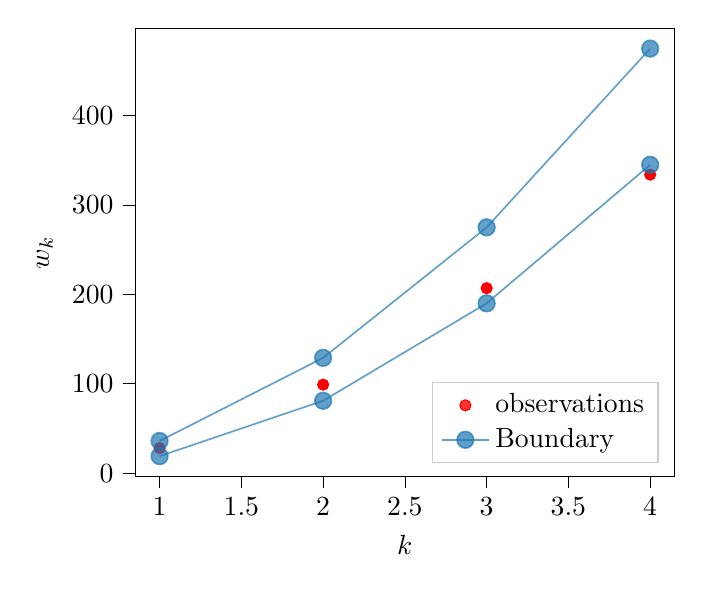
\begin{tikzpicture}

\definecolor{darkgray176}{RGB}{176,176,176}
\definecolor{lightgray204}{RGB}{204,204,204}
\definecolor{steelblue31119180}{RGB}{31,119,180}

\begin{axis}[
legend cell align={left},
legend style={
  fill opacity=0.8,
  draw opacity=1,
  text opacity=1,
  at={(0.97,0.03)},
  anchor=south east,
  draw=lightgray204
},
tick align=outside,
tick pos=left,
x grid style={darkgray176},
xlabel={\(\displaystyle k\)},
xmin=0.85, xmax=4.15,
xtick style={color=black},
y grid style={darkgray176},
ylabel={\(\displaystyle w_k\)},
ymin=-3.8, ymax=497.8,
ytick style={color=black}
]
\addplot [draw=red, fill=red, mark=*, only marks]
table{%
x  y
1 28
2 99
3 207
4 334
};
\addlegendentry{observations}
\addplot [semithick, steelblue31119180, opacity=0.7, mark=*, mark size=3, mark options={solid}]
table {%
1 19
2 81
3 190
4 345
};
\addlegendentry{Boundary}
\addplot [semithick, steelblue31119180, opacity=0.7, mark=*, mark size=3, mark options={solid}, forget plot]
table {%
1 36
2 129
3 275
4 475
};
\end{axis}

\end{tikzpicture}

\caption{Illustration of the boundary.\label{fig:gst}}
\end{center}
\end{figure}

\subsection{Permutation tests}
Permutation tests are non-parametric tests that are ...

\subsection{Multiple testing}
When dealing with multiple testing, particular care must be taken so as not to decrease the error of the test. Suppose that we want to test $H_j$ versus $H_j'$ for $1\le j\le J$ using a test statistic $T_{N}^{(j)}$. Instead of the type I error considered in two-sample testing, we consider the family-wise error rate (FWE) which is defined as the probability of making at least one type I error: let $\textbf{I}\subset \{1,\dots,J\}$ be the set of the true hypotheses, then 
$$\mathrm{FWE} = \P_{H_j, j \in \textbf{I}}\left(\exists j \in \textbf{I}:\quad  \text{reject }H_j \right).$$
Usually, we say that an algorithm has a weak FWE control if the FWE is smaller than $\alpha$ when $\textbf{I}=\{1,\dots,J\}$ and we say that the algorithm has strong FWE control if FWE is smaller than $\alpha$ for any $\textbf{I}\neq \emptyset$.

There are several procedures that can be used to have control on the FWE. The most famous one is Bonferroni procedure, it is a very simple procedure in which we take a threshold for $H_j$ vs $H_j'$ equal to a quantile of order $1-\alpha/J$ of the permutation distribution of $T_n^{(j)}$. It can be very conservative in general and we will prefer a step-down method that performs better in practice.

\paragraph{Step-down procedure:} proposed by \cite{Romano_2003}, the step-down procedure is defined as follows: for some $\textbf{C} \subset \{1,\dots,J\}$, denote
$$T_{n}^{(\textbf{C})}(\sigma)= \max\left(T_n^{(j)}(\sigma),\quad j \in \textbf{C}\right)$$
\begin{algorithm}[h]
\SetAlgoLined
\SetKwInput{KwParameter}{Parameters}
\KwParameter{$\alpha \in (0,1)$}
Initialize $\textbf{C}=\{1,\dots,J\}$\\
\While{$\textbf{C} \neq \emptyset$}{
Compute $\widehat{b}_{n}^{(\textbf{C})}(1-\alpha)$ the quantile of order $1-\alpha$ of the permutation law of $T_{n}^{(\textbf{C})}(\sigma)$:
$$\sum_{\sigma \in \S_{2n}} \1\{T_{n}^{(\textbf{C})}(\sigma) \ge  \widehat{b}_{n}^{(\textbf{C})}\} = \lfloor \alpha n! \rfloor .$$
\uIf{$T_{n}^{(\textbf{C})}(\mathrm{id}) \le \widehat{b}_{n}^{(\textbf{C})}$}{
Accept all the hypotheses $H_j, j\in \textbf{C}$ and break the loop.}
\Else{
Reject $H_{j_{\max}}$ where $j_{\max} =  \arg\max\left(T_n^{(j)}(\sigma),\quad j \in \textbf{C}\right)$.\\
Define $\textbf{C}=\textbf{C} \setminus \{j_{max}\}$
}
}
\caption{Multiple testing, non-sequential.}\label{alg:multiple_test_1}
\end{algorithm}
The Algorithm~\ref{alg:multiple_test_1} is consistent (i.e. $\mathrm{FWE}\le \alpha$) for the equality of distribution hypotheses. It uses the maximum of the statistics as a mean to test an intersection of hypotheses. This procedure is not specific to permutation tests and can be used for other tests provided some properties on the thresholds $\widehat{b}_{n}^{(\textbf{C})}$. 


Remark that we could not use Benjamini-Hochberg procedure or similar procedures because the hypotheses are not independent. We adapt this procedure to the case of group sequential testing in Section~\ref{sec:main_algo}

\subsection{Random permutation to speed up computation}
We use Monte-Carlo approximation, using random permutation instead of enumerating all the permutations.
\section{Main algorithm}\label{sec:main_algo}

\subsection{Notations}
We denote by $\S_{2N}$ the set of permutations of $\{1,\dots,2N\}$ and for $\sigma_1,\sigma_2,\dots,\sigma_k \in \S_{2N}^2$, we denote $\sigma_1 \cdot \sigma_2 \cdot \ldots \cdot \sigma_k$ the concatenation of the permutation $\sigma_1$ done in interim $1$ and $\sigma_2$ done on interim $2$,\dots, $\sigma_k$ on interim $k$. We consider $L\ge 2$ agents $A_1,\dots,A_L$. The $k^{th}$ step of the algorithm is called the $k^{th}$ interim for some $k \in \{1,\dots,K\}$. Let $c_1,\dots,c_J$ be the comparisons we want to make. For any $i$, $c_i$ is a couple of agent's indices: $c_i=(c_{i,1},c_{i,2}) \in \{1,\dots,L\}^2$. We denote $e_{1,k}(j), \dots, e_{2N, k}(j)$ the concatenation of the $2N$ evaluations obtained from the two agents compared for comparison $j$ at at interim $k$.

For some $\textbf{C} \subset \{1,\dots,J\}$, denote
$$T_{N,k}^{(\textbf{C}^+)}(\sigma)= \max\left(T_{N,k}^{(j)}(\sigma),\quad j \in \textbf{C}\right) \quad \text{and}\quad T_{N,k}^{(\textbf{C}^-)}(\sigma)= \min\left(T_{N,k}^{(j)}(\sigma),\quad j \in \textbf{C}\right)$$
where 
$$T_{N,i}^{(j)}(\sigma)= \left|\sum_{i=1}^k\left(\sum_{n=1}^{N} e_{\sigma_i(n),i}(j)-\sum_{n=N+1}^{2N} e_{\sigma_i(n),i}(j)\right)\right|$$ 
$T_{N,i}^{(j)}$ is the absolute value of the sum of differences of all the blocks until block $i$ after permutation of the concatenation of the two agents's evaluations. by $\sigma_1,\dots,\sigma_i\in \S_{2N}$.
 
$\textbf{I}$ denotes the set of indices of the true hypotheses among $\{1,\dots,J\}$. Let $\alpha, \beta \in [0,1]$, the algorithm depends on a level spending function $f^+:[0,1]\to[0,\alpha]$ and a power spending function $f^-:[0,1]\to [0,\beta]$, both non-decreasing functions verifying $f^+(0)=f^-(0)=0$, $f^+(1)=\alpha$, $f^-(1)=\beta$. 

If $\textbf{I} \neq \emptyset$, we denote 
$$\mathrm{FWE}(\alpha) = \P\left(\exists j \in \textbf{I}:\quad  \text{reject }H_j \right).$$
\subsection{AdaStop: adaptive stopping algorithm using step-down method and group sequential permutation tests}

The algorithm is given in Algorithm~\ref{algo:main}
\begin{algorithm}[h]
\SetAlgoLined
\SetKwInput{KwParameter}{Parameters}
\KwParameter{Agents $A_1,A_2,\dots, A_L$, environment $\mathcal{E}$, comparison pairs $(c_i)_{i \le L}$ where $c_i$ is a couple of two agents that we want to compare. Integers $K,N \in \N^*$, test parameters $\alpha,\beta$.}
Define $LNK$ different seeds $(s_{l,n,k})_{l\le L,n\le N, k\le K}$.\\
Set $\textbf{C}=\{1, \dots,L\}$ the set of indices for the comparisons we want to do.\\
\For{$k=1,\dots,K$}{
\For{$l=1...L$}{
Train agent $A_l$ on environment $\mathcal{E}$ with the seeds $s_{l,1,k},\dots,s_{l,N,k}$.\\
Collect the $N$  evaluations of agent $A_l$.\\
}
Set $\lambda^+ = f^+ \left(\frac{k}{K}\right)- f^+ \left( \frac{k-1}{K}\right)$ and $\lambda^- = f^- \left(\frac{k}{K}\right)- f^- \left( \frac{k-1}{K}\right)$.\\

\While{True}{
Compute the boundary $\widehat{b}_{N,k}^{(\textbf{C}^+)}$ and $\widehat{b}_{N,k}^{(\textbf{C}^-)}$ such that
$$\frac{1}{((2N)!)^k}\sum_{\sigma \in S_k} \1\{T_{N,k}^{(\textbf{C}^+)}(\sigma) \ge  \widehat{b}_{N,k}^{(\textbf{C}^+)}\} \le  \lambda^+ \quad \text{and}\quad \frac{1}{((2N)!)^k}\sum_{\sigma \in S_k} \1\{T_{N,k}^{(\textbf{C}^-)}(\sigma) \leq   \widehat{b}_{N,k}^{(\textbf{C}^-)}\} \le  \lambda^-  .$$
where $S_k$ is the set of permutations $\sigma\in(\S_{2N})^k$  such that it would not have accepted or rejected before
$$\forall m < k,\quad  T_{N,m}^{(\textbf{C}^+)}(\sigma) \le   \widehat{b}_{N,m}^{(\textbf{C}^+)} \text{ and }T_{N,m}^{(\textbf{C}^-)}(\sigma) \ge   \widehat{b}_{N,m}^{(\textbf{C}^-)} $$

\uIf{$T_{N,k}^{(\textbf{C}^+)}(\mathrm{id}) > \widehat{b}_{N,k}^{(\textbf{C}^+)}$}{
Reject $H_{j_{\max}}$ where $j_{\max} =  \arg\max\left(T_{N,k}^{(j)}(\id),\quad j \in \textbf{C}\right)$.\\
Update $\textbf{C}=\textbf{C} \setminus \{j_{\max }\}$
}
\uElseIf{$T_{n,k}^{(\textbf{C}^-)}(\mathrm{id}) < \widehat{b}_{N,k}^{(\textbf{C}^-)}$}{
Accept $H_{j_{\min}}$ where $j_{\min} =  \arg\min\left(T_{N,k}^{(j)}(\id ),\quad j \in \textbf{C}\right)$.\\
Update $\textbf{C}=\textbf{C} \setminus \{j_{\min }\}$
}
\Else{ break the while loop
}
}
\lIf{$\textbf{C}=\emptyset$}{
Break the loop and returns the answers
}
{
\lIf{ $k=K$}{
 Then accept all hypotheses remaining in $\textbf{C}$ and break the loop
}
}
}
\caption{Main algorithm\label{algo:main}}
\end{algorithm}

\newpage

\section{Theoretical guarentees}
% \todoT{For now: asymptotic is not with early accept and not multiple.}
% \todoT{
% TODO:\\
% - Prove that early accept does not decrease the power too much\\
% - Do the asymptotic for early accept and multiple testing (this would also allow estimate of power)
% } 
\subsection{Basic results following from the use of permutation tests}
One of the basic property of two-sample permutation tests is that when the null hypothesis is true, then all the permutation are as likely to give a certain value and hence the law given the data is the uniform distributions on all the permutations. The precise theorem for this result is a bit technical due to the fact that the probability for the data to have any given value is $0$ and we must be a bit careful with the formulation (see \cite[Theorem 17.2.2]{lehmann2005testing} for a precise formulation). 

In what follows we show results with the same flavour but adapted to our multi-testing and sequential testing problem to fit exactly our setting.
\begin{Lemma}\label{lem:quantile_permu_2}
Let $X_1,\dots,X_N$ be i.i.d from a distribution $P$ and $Y_1,\dots,Y_N$ be i.i.d. from a distribution $Q$. Denote $Z_1^{2N}=X_1,\dots,X_N,Y_1,\dots,Y_N$ be the concatenation of $X_1^N$ and $Y_1^N$. Let $\alpha \in (0,1)$ and define $\widehat{b}$ such that 
$$ \frac{1}{(2N)!}\sum_{\sigma\in \S_{2N}} \1\left\{ \frac{1}{N}\sum_{i=1}^n (Z_{\sigma(i)}-Z_{\sigma(N+i)}) > \widehat{b}\right\}\le \alpha.$$
Then, if $P=Q$, we have 
$$\P\left(\frac{1}{N}\sum_{i=1}^n (X_i-Y_i) >\widehat{b} \right)\le \alpha $$ 
\end{Lemma}
\begin{proof}
Denote $T(\sigma)= \frac{1}{N}\sum_{i=1}^n (Z_{\sigma(i)}-Z_{\sigma(n+i)})$ and $\P$ be the probability with respect to the laws of $X_1^N$ and $Y_1^N$. Since $P=Q$, for any $\sigma,\sigma' \in \S_{2N}$ we have $T(\sigma)=^d T(\sigma')$. Then, because $\widehat{b}$ does not depend on the permutation $\sigma$ (but it depends on the values of $Z_1^{2N}$, we have for any $\sigma \in \S_{2N}$
\begin{align*}
\P\left(T(\id)> \widehat{b}\right)&=\P\left(T(\sigma)> \widehat{b}\right)
\end{align*} 
Now, take the sum on all the permutations, 
\begin{align*}
\P\left(T(\id)> \widehat{b}\right)&=\frac{1}{(2N)!}\sum_{\sigma\in \S_{2N}} \E\left[\1\{T(\sigma)> \widehat{b}\}\right]\\
&=  \E\left[\frac{1}{(2N)!}\sum_{\sigma\in \S_{2N}}\1\{T(\sigma)> \widehat{b}\}\right]\le \alpha
\end{align*}
which proves the result.
\end{proof}


More generally, Lemma~\ref{lem:quantile_permu_2} is true even for more general permutation tests. In particular, in our case we have

\begin{Lemma}
for any $j \in \textbf{I}$, then we have the following joint equality in distribution :
$$\forall \sigma \in (\S_{2N})^k, \quad (T_N^{(j)}(\id))_{j \in\textbf{I}} =^d (T_N^{(j)}(\sigma))_{j \in \textbf{I}}.$$
where $\textbf{I}$ is a subset of $\{1,\dots,J\}$ of true hypotheses.
\end{Lemma}
\begin{proof}
We have
\begin{align*}
T_{N,k}^{(j)}(\sigma_1 \cdot  \sigma_2 \cdot  \ldots  \cdot  \sigma_k)&=  \left|\sum_{i=1}^k\left(\sum_{n=1}^{N} e_{\sigma_i(n),i}(j)-\sum_{n=N+1}^{2N} e_{\sigma_i(n),i}(j)\right)\right|
\end{align*}
Hence, $T_{N,k}^{(j)}(\sigma) = T_{N,k}^{(j)}(\sigma')$ where $\sigma'_i(n)=\sigma_i(n+N)$ if $n \le N$ and $\sigma_i(n) = \sigma_i(n-N)$ otherwise. This corresponds to changing the sign $-1$ to $+1$ inside the absolute value. Now, let us consider two different comparisons $j=(i_1,i_2)$ and $j'=(i_2,i_3)$, i.e. the two couples share one agent. We can consider that in both $T_{N,k}^{(j)}(\sigma)$ and $T_{N,k}^{(j')}(\sigma)$ the permutation acts in the same way on agent $i_2$.

As a consequence transformation by $\sigma$ can be seen as a global transformation of the concatenation of all the points (with repetition removed) $(e_{n,i}(j), e_{n,i}(j))_{n\le N, i\le k,j\in \textbf{I}}$. 

Now, we define the connected clusters of indices in $\textbf{I}$. We denote $\mathcal{C}(i)$ the connected cluster of agent $i \in \{1,\dots,L\}$ which consists in all the agents that are compared to it in $\textbf{I}$: $\mathcal{C}(i)=\{l \in  \{1,\dots,L\}:\quad  (l,i)\in \textbf{I}\}$ where $(l,i)$ is taken without order. Because the agents's evaluations are independent from one-another, the cluster of indices are also independent and we can consider them separately. 

In each cluster, as said previously, we can consider that the data are transform by a global permutation on the indices, and the permutation must be of the form of a concatenation of permutations on interims as defined previously. Then, because the samples are i.i.d because we consider only true hypotheses, using the usual permuted exchangeability argument  we get that for all $i$, $(T_N^{(j)}(\id))_{j \in\textbf{C(i)}} =^d (T_N^{(j)}(\sigma))_{j \in \textbf{C(i)}}$, then we get the result because the clusters are independent.
\end{proof}

% By convention, let $f^+\left(\frac{-1}{K}\right)=0$. We have,
% \begin{Lemma}
% Let $(X_{i,j})_{i\le n, j\le J}$ be i.i.d from a distribution $P_1,\dots,P_J$. Let $\textbf{I}$ be a set of comparisons $(i,j)$ for which we have $P_i=P_j$ is true. Let $\alpha \in (0,1)$ and define $\widehat{b}_{n}^{(\textbf{I}^+)}$ as in Algorithm~\ref{algo:main}, we have
% $$\P\left(T_{N,k}^{(\widehat{\textbf{I}}_k^+)}(\id) > \widehat{b}_{N,k}^{(\widehat{\textbf{I}}_k^+)}\Big| \forall m < k  \quad T_{N,m}^{(\textbf{I}^+)}(\sigma) \le   \widehat{b}_{N,m}^{(\textbf{I}^+)}\right)\le f^{+}\left(\frac{k}{K}\right)- f^{+}\left(\frac{k-1}{K}\right).$$
% \end{Lemma}
% \begin{proof}
% For  $\textbf{J}\subset \textbf{I}$,  denote 
% $$E_k(\sigma,\textbf{J}) = \left\{\forall m < k, T_{N,m}^{(\textbf{I}^+)}(\sigma) \le   \widehat{b}_{N,m}^{(\textbf{I}^+)} \text{ and }T_{N,m}^{(\textbf{J}^-)}(\sigma) \ge   \widehat{b}_{N,m}^{(\textbf{J}^-)}\right\}$$
% which correspond to the event  ``did not reject any true hypotheses and did nor accept any $H_j$ for $j  \in \textbf{J}$ before interim k after permutation by $\sigma$''.  Denote by $\textbf{C}_k$ the (random) value of $\textbf{C}$ at the beginning of interim $k$. 
% We have
% \begin{align*}
% \P&\left(T_{N,k}^{(\textbf{C}_k^+)}(\id) > \widehat{b}_{N,k}^{(\textbf{C}_k^+)}, \forall m < k  \quad T_{N,m}^{(\textbf{I}^+)}(\id) \le   \widehat{b}_{N,m}^{(\textbf{I}^+)} \right)\\
% &= \P\left(T_{N,k}^{(\textbf{C}_k^+)}(\id) > \widehat{b}_{N,k}^{(\textbf{C}_k^+)} , \forall m < k  \quad T_{N,m}^{(\textbf{I}^+)}(\id) \le   \widehat{b}_{N,m}^{(\textbf{I}^+)}\right) \\
% &=\P\left(\max\{ T_{N,k}^{(j)}(\id), j \in \textbf{C}_k\} > \widehat{b}_{N,k}^{(\textbf{C}_k^+)} , E_k(\id,\textbf{C}_k)\right)
% \end{align*}

% Let $\widehat{\textbf{I}}_k$ the (random) set of true hypotheses not yet accepted or rejected at interim $k$. Remark that having that on the event $E_k(\sigma,J)$, we never rejected any hypothesis from $\textbf{I}$ before interim $k$, and interim $k$ correspond to a reject of an hypothesis from $\textbf{I}_k$: there exists $ \widehat{j} \in \textbf{I}_k$ such that $\max\{ T_{N,k}^{(j)}(\id), j \in\textbf{C}_k\} = T_{N,k}^{(\widehat{j})}(\id)$. Hence, we have
% $$\max\{ T_{N,k}^{(j)}(\id), j \in\textbf{C}_k\} =\max\{ T_{N,k}^{(j)}(\id ), j \in \widehat{\textbf{I}}_k\}. $$

% And moreover, we also have that at interim $k$, $\textbf{C}_k \supset \widehat{\textbf{I}}_k$ because initially $\textbf{I} \subset \textbf{C}_1$ and any accepted hypotheses were removed from both $\textbf{C}_1$ and from $\textbf{I}$ to give $\textbf{C}_k$ and  $\widehat{\textbf{I}}_k$ respectively. Hence
% $\widehat{b}_{N,k}^{(\textbf{C}_k^+)} \ge \widehat{b}_{N,k}^{(\widehat{\textbf{I}}_k^+)} $, and we have 

% \begin{align*}
% \1\left\{\max\{ T_{N,k}^{(j)}(\id), j \in \textbf{C}_k\} > \widehat{b}_{N,k}^{(\textbf{C}_k^+)},  E_k(\id, \textbf{C}_k)\right\}  &\le \1\left\{\max\{ T_{N,k}^{(j)}(\id), j \in \widehat{\textbf{I}}_k\} > \widehat{b}_{N,k}^{(\widehat{\textbf{I}}_k^+)}\right\}
% \end{align*}
% Hence,
% \begin{align*}
% \P\left(T_{N,k}^{(\textbf{C}_k^+)}(\id) > \widehat{b}_{N,k}^{(\textbf{C}_k^+)}, \forall m < k  \quad T_{N,m}^{(\textbf{I}^+)}(\id) \le   \widehat{b}_{N,m}^{(\textbf{I}^+)} \right)&\le \P\left(\max\{ T_{N,k}^{(j)}(\id), j \in \widehat{\textbf{I}}_k\} > \widehat{b}_{N,k}^{(\widehat{\textbf{I}}_k^+)} \right)
% \end{align*}


% Then, then we have the joint equality in distribution $(T_N^{(j)}(\id))_{j \in\textbf{I}} =^d (T_N^{(j)}(\sigma))_{\textbf{I}}$ for any $\sigma \in (\S_{2N})^k$. 
% \begin{align*}
% \P\left(T_{N,k}^{(\textbf{C}_k^+)}(\id) > \widehat{b}_{N,k}^{(\textbf{C}_k^+)}, \forall m < k  \quad T_{N,m}^{(\textbf{I}^+)}(\id) \le   \widehat{b}_{N,m}^{(\textbf{I}^+)} \right)&\le \frac{1}{((2N)!)^k}\sum_{\sigma_1,\dots,\sigma_k \in \S_{2N}}\P\left(\max\{ T_{N,k}^{(j)}(\sigma), j \in \widehat{\textbf{I}}_k\} > \widehat{b}_{N,k}^{(\widehat{\textbf{I}}_k^+)} \right)
% \end{align*}


% \begin{align*}
% \P&\left(\max\{ T_{N,k}^{(j)}(\id), j \in \textbf{J}\} > \widehat{b}_{N,k}^{(\textbf{J}^+)} ,\textbf{J} = \textbf{C}_k, E_k(\id,\textbf{J})\right)\\
% &= \frac{1}{((2N)!)^k}\sum_{\sigma_1,\dots,\sigma_k \in \S_{2N}} \P\left(\max\{ T_{N,k}^{(j)}(\sigma), j \in \textbf{J}\} > \widehat{b}_{N,k}^{(\textbf{J}^+)} ,  \textbf{J} = \textbf{C}_k,E_k(\sigma,\textbf{J})\right)\\
% &= \frac{1}{((2N)!)^k} \E\left[\sum_{\sigma_1,\dots,\sigma_k \in \S_{2N}}\1\left\{\max\{ T_{N,k}^{(j)}(\sigma), j \in \textbf{J}\} > \widehat{b}_{N,k}^{(\textbf{J}^+)} , \textbf{J} = \textbf{C}_k,E_k(\sigma,\textbf{J})\right\}\right]\\
% \end{align*}
% \begin{align*}
% \P&\left(\max\{ T_{N,k}^{(j)}(\id), j \in \textbf{J}\} > \widehat{b}_{N,k}^{(\textbf{J}^+)} ,\textbf{J} = \widehat{\textbf{I}}_k, E_k(\id,\textbf{J})\right)\\
% &\le  \left(f^{+}\left(\frac{k}{K}\right)- f^{+}\left(\frac{k-1}{K}\right)\right)\E\left[\frac{1}{((2N)!)^k} |S_k|\1\{\textbf{J} = \widehat{\textbf{I}}_k\}\right]\\
% &=  \left(f^{+}\left(\frac{k}{K}\right)- f^{+}\left(\frac{k-1}{K}\right)\right)\E\left[\frac{1}{((2N)!)^k} \sum_{ \sigma_1,\dots,\sigma_k \in \S_{2N}}\1\{E_k(\sigma, \textbf{J}), \textbf{J} = \widehat{\textbf{I}}_k\}\right]\\
% &= \left(f^{+}\left(\frac{k}{K}\right)- f^{+}\left(\frac{k-1}{K}\right)\right)\frac{1}{((2N)!)^k} \sum_{ \sigma_1,\dots,\sigma_k \in \S_{2N}} \P(E_k(\sigma, \textbf{J}), \textbf{J} = \widehat{\textbf{I}}_k )\\
% &= \left(f^{+}\left(\frac{k}{K}\right)- f^{+}\left(\frac{k-1}{K}\right)\right)
%  \P(E_k(\id, \textbf{J}), \textbf{J} = \widehat{\textbf{I}}_k )\\
% &\le \left(f^{+}\left(\frac{k}{K}\right)- f^{+}\left(\frac{k-1}{K}\right)\right)
%  \P( \textbf{J} = \widehat{\textbf{I}}_k )
% \end{align*}
% Hence,
% \begin{align*}
% \P\left(T_{N,k}^{(\widehat{\textbf{I}}_k^+)}(\id) > \widehat{b}_{N,k}^{(\widehat{\textbf{I}}_k^+)} \right)&= \sum_{ \textbf{J}\subset \textbf{I} }\P\left(\max\{ T_{N,k}^{(j)}(\id), j \in \textbf{J}\} > \widehat{b}_{N,k}^{(\textbf{J}^+)} ,  E_k(\id,\textbf{J}), \textbf{J} = \widehat{\textbf{I}}_k\right)\\
% &\le \sum_{ \textbf{J}\subset \textbf{I} }\left(f^{+}\left(\frac{k}{K}\right)- f^{+}\left(\frac{k-1}{K}\right)\right)\P( \textbf{J} = \widehat{\textbf{I}}_k ) \\
% &= f^{+}\left(\frac{k}{K}\right)- f^{+}\left(\frac{k-1}{K}\right).
% \end{align*}
% \end{proof}



\subsection{Multiple group sequential testing}
First we prove that the multiple testing scheme is correct for testing $ P_j = P_k$ against $ P_j \neq P_k$ for all the couples $j \neq k$. 


\begin{Theorem}\label{th:multi_FWE}
Suppose that $\beta = 0$, for any $\alpha \in (0,1)$ and any non-decreasing level spending function $f^+$, the test resulting from Algorithm~\ref{algo:main} has a strong control on the FWE: we have $\mathrm{FWE}(\alpha)\le\alpha$.
\end{Theorem}
\begin{proof}
Denote 
$$E_k(\sigma) = \left\{\forall m < k,\quad  T_{N,m}^{(\textbf{I}^+)}(\sigma_1\cdot\ldots\cdot\sigma_m) \le   \widehat{b}_{N,m}^{(\textbf{I}^+)}\right\}$$
Denote by $\textbf{C}_k$ the (random) value of $\textbf{C}$ at the beginning of interim $k$. 


Let $\textbf{I}$ be the set of true hypotheses. Let A be the following event
$$\mathrm{A}= \{ \exists j \in \textbf{I}: \quad H_j \text{ is rejected}\}.$$
We have 
\begin{align*}\label{eq:multi1}
\P_\sigma\left(\text{A is true} \right)&= \sum_{k=1}^K \P\left( \exists j \in \textbf{I}: \quad H_j\text{ is rejected at interim $k$ }|\text{there were no rejection before interim $k$}\right)\\
&\le   \sum_{k=1}^K  \P\left(\exists \textbf{J}:\quad  T_{N,k}^{(\textbf{J}^+)}(\id) > \widehat{b}_{N,k}^{(\textbf{J}^+)}, E_k(\id), \arg\max_{j \in \textbf{J}}T_{N,k}^{(j)}(\id) \in \textbf{I}, \forall \textbf{C}_k \supset \textbf{J}'\supsetneq\textbf{J} \quad  \arg\max_{j \in \textbf{J}'}T_{N,k}^{(j)}(\id) \notin \textbf{I} \right)
\end{align*}
$E_k(\id)$ means that we look at the first interim that rejects, $\arg\max_{j \in \textbf{J}}T_{N,k}^{(j)}(\id) \in \textbf{I}$ means that we reject a true hypothesis, and $\forall \textbf{C}_k \supset \textbf{J}'\supsetneq \textbf{J} \quad  \arg\max_{j \in \textbf{J}'}T_{N,k}^{(j)}(\id) \notin \textbf{I} $ means that $\textbf{J}$ corresponds to the set for the first rejection of a true hypothesis (there can be several rejection of false hypotheses before but not rejection of a true hypothesis). 
We denote 
$$\mathrm{FWE}_k =  \P\left(\exists \textbf{J}:\quad  T_{N,k}^{(\textbf{J}^+)}(\id) > \widehat{b}_{N,k}^{(\textbf{J}^+)}, E_k(\id), \arg\max_{j \in \textbf{J}}T_{N,k}^{(j)}(\id) \in \textbf{I}, \forall \textbf{C}_k \supset \textbf{J}'\supsetneq\textbf{J} \quad  \arg\max_{j \in \textbf{J}'}T_{N,k}^{(j)}(\id) \notin \textbf{I} \right),$$ 
the error of interim $k$ and by convention we take $f^+(-1/K)=0$.

%  \paragraph{First interim:}
% the first interim is a non-sequential test, the result follows from (cite Exact and Approximate Stepdown Methods for Multiple Hypothesis Testing). We include here a proof with our notations for completness and as an introduction to the proof of the other interim.

% After the first interim, $\textbf{C}_1 = \{1,\dots,J\}$ and $E_1(\id)$ is always true. We have in the case of type I error, 
% \begin{align*}
% \mathrm{FWE}_1 &= \P\left( T_{N,1}^{(\textbf{J}^+)}(\id) > \widehat{b}_{N,1}^{(\textbf{J}^+)}, E_1(\id), \arg\max_{j \in \textbf{J}}T_{N,1}^{(j)}(\id) \in \textbf{I}, \forall \textbf{C}_1 \supset \textbf{J}'\supsetneq \textbf{J} \quad  \arg\max_{j \in \textbf{J}'}T_{N,1}^{(j)}(\id) \notin \textbf{I} \right)\\
% &=\P\left( T_{N,1}^{(\textbf{J}^+)}(\id) > \widehat{b}_{N,1}^{(\textbf{J}^+)},  \arg\max_{j \in \textbf{J}}T_{N,1}^{(j)}(\id) \in \textbf{I}, \forall  \textbf{J}'\supsetneq \textbf{J} \quad  \arg\max_{j \in \textbf{J}'}T_{N,1}^{(j)}(\id) \notin \textbf{I} \right)
% \end{align*}
% remark that because $\textbf{J}$ is the first rejection of a true hypothesis to occure, we have on the event 
% $$\{ \arg\max_{j \in \textbf{J}}T_{N,1}^{(j)}(\id) \in \textbf{I}, \forall  \textbf{J}'\supsetneq \textbf{J} \quad  \arg\max_{j \in \textbf{J}'}T_{N,1}^{(j)}(\id) \notin \textbf{I}\} $$
% that
% $$T_{N,1}^{(\textbf{J}^+)}(\id)= \max\{T_{N,1}^{(j)}(\id), j \in \textbf{J}\} = \max\{T_{N,1}^{(j)}(\id), j \in \textbf{I}\} = T_{N,1}^{(\textbf{I}^+)}(\id)$$
% Moreover, we $\textbf{J} \supset \textbf{I}$ because no true hypothesis have been rejected or accepted before, hence $\widehat{b}_{N,1}^{(\textbf{J}^+)} \ge \widehat{b}_{N,1}^{(\textbf{I}^+)}$. And finally, we have 
% \begin{align*}
% \mathrm{FWE}_1\le \P\left( T_{N,1}^{(\textbf{I}^+)}(\id) > \widehat{b}_{N,1}^{(\textbf{I}^+)} \right)
% \end{align*}
% now, because we are only dealing with true hypotheses, we can apply the invariance principle which assure the joint equality in distribution of $(T_{N,1}^{(j)}(\id))_{j \in \textbf{I}}$ and $( T_{N,1}^{(j)}(\sigma_1))_{j \in \textbf{I}}$ for any $\sigma_1 \in \S_{2N}$ to have
% \begin{align*}
% \mathrm{FWE}_1&\le \frac{1}{(2N)!}\sum_{\sigma_1 \in \S_{2N}}\P\left( T_{N,1}^{(\textbf{I}^+)}(\sigma_1) > \widehat{b}_{N,1}^{(\textbf{I}^+)} \right)\\
% &= \E\left[\frac{1}{(2N)!}\sum_{\sigma_1 \in \S_{2N}}\1\left\{ T_{N,1}^{(\textbf{I}^+)}(\sigma_1) > \widehat{b}_{N,1}^{(\textbf{I}^+)}\right\} \right]\le f^+\left(\frac{1}{K}\right)
% \end{align*}
% the last inequality follows by definition of $\widehat{b}_{N,1}^{(\textbf{I}^+)}$.
% \paragraph{Interim $1<k\le  K$:}

Remark that on $$E_k(\id) \cap \{\arg\max_{j \in \textbf{J}}T_{N,k}^{(j)}(\id) \in \textbf{I}\}\cap\{ \forall \textbf{C}_k \supset \textbf{J}'\supsetneq\textbf{J} \quad  \arg\max_{j \in \textbf{J}'}T_{N,k}^{(j)}(\id) \notin \textbf{I}\}  $$
$\textbf{J}$ corresponds to the first rejection to occur. Hence, having that the argmax is attaind in $\textbf{I}$,
$$T_{N,k}^{(\textbf{J}^+)}(\id)= \max\{T_{N,k}^{(j)}(\id), j \in \textbf{J}\} = \max\{T_{N,1}^{(j)}(\id), j \in \textbf{I}\} = T_{N,k}^{(\textbf{I}^+)}(\id)$$
Moreover, we $\textbf{J} \supset \textbf{I}$ because no true hypothesis have been rejected or accepted before, hence $\widehat{b}_{N,k}^{(\textbf{J}^+)} \ge \widehat{b}_{N,k}^{(\textbf{I}^+)}$. And finally, we have 
\begin{align*}
\mathrm{FWE}_k\le \P\left( T_{N,k}^{(\textbf{I}^+)}(\id) > \widehat{b}_{N,k}^{(\textbf{I}^+)}, E_k(\id) \right)
\end{align*}
now, because we are only dealing with true hypotheses, we can apply the invariance principle from Lemma~\ref{lem:invariance} which assure the joint equality in distribution of $(T_{N,1}^{(j)}(\id))_{j \in \textbf{I}}$ and $( T_{N,1}^{(j)}(\sigma))_{j \in \textbf{I}}$ for any $\sigma \in (\S_{2N})^k$ to have
\begin{align*}
\mathrm{FWE}_k &\le \frac{1}{((2N)!)^k}\sum_{\sigma_1,\dots,\sigma_k \in \S_{2N}}\P\left( T_{N,k}^{(\textbf{I}^+)}(\sigma) > \widehat{b}_{N,k}^{(\textbf{I}^+)}, E_k(\sigma) \right)\\
&= \E\left[\frac{1}{((2N)!)^k}\sum_{\sigma \in (\S_{2N})^k}\1\left\{ T_{N,k}^{(\textbf{I}^+)}(\sigma) > \widehat{b}_{N,k}^{(\textbf{I}^+)}, E_k(\sigma)\right\} \right]\\
&\le \E\left[\frac{1}{((2N)!)^k}\sum_{\sigma \in (S_k)^k}\1\left\{ T_{N,k}^{(\textbf{I}^+)}(\sigma) > \widehat{b}_{N,k}^{(\textbf{I}^+)}\right\} \right]\\
&\le f^+\left(\frac{k}{K}\right)-f^+\left(\frac{k-1}{K}\right)\\
\end{align*}
the last inequality follows by definition of $\widehat{b}_{N,k}^{(\textbf{I}^+)}$.
\end{proof}
To control the FWE, we only care about true hypotheses $j \in \textbf{I}$. Let $\beta>0$ and consider a comparison $j \in \textbf{I}$ that have been stopped early. If it had not been stopped, it could have been wrongly rejected, increasing the error. Hence the type I error can only decrease when we accept early. The consequence of early accept is an increase in type II error.
\begin{Lemma}
The familywise-error rate is smaller when we use early-accept ($\beta>0$) than when we do not.
\end{Lemma}

% \newpage
\section{Offline experimental comparison with the litterature}
\todoT{Comparison with edge of statistical precipice and Flower's team article}
\section{Online experimental results}
\todoT{Test to compare PPO and other}
\appendix

\section{Non-sequential permutation test}

Foor a sample $Z_1^n=(Z_1,\dots,Z_n)$, denote $\sigma Z_1^n$ the permuted sample using the permutation $\sigma$: $\sigma Z_1^n=(Z_{\sigma(1)},\dots,Z_{\sigma(n)})$.\\
For $T_n$ the difference of empirical mean, we have the following property.

\begin{Proposition}\label{prop:asym_perm_test}
Let $T_n(Z_1,\dots,Z_{2n})=\frac{1}{\sqrt{n}}\sum_{i=1}^n Z_i -\frac{1}{n}\sum_{i=n+1}^{2n} Z_i$.

Suppose $X_1,\dots,X_n$ are i.i.d from $P$ and $Y_1,\dots,Y_n$ are i.i.d from $Q$ and both $P$ and $Q$ has finite variance. Denote $Z_1,\dots,Z_{2n}=X_1,\dots,X_n, Y_1,\dots,Y_n$ the concatenation of the two samples. Then, we have
$$\sup_{t}\left|\frac{1}{n!}\sum_{\sigma \in \S_{2n}} \1\{T_n(\sigma Z_{1}^{2n}) \le t\}- \Phi\left(t/\tau(P,Q) \right)\right|\xrightarrow[n \to \infty]{P} 0$$
where $\tau(P,Q)^2=\sigma_P^2+\sigma_Q^2+\frac{(\mu_P- \mu_Q)^2}{2} $.
\end{Proposition}
Remark: this proposition can be extended to other $T_n$ statistics using Theorem 2.1 in \cite{Chung_2013} or Theorem 15.2.5 of \cite{lehmann2005testing}.
%\todoT{Maybe I could do an edgeworth expansion to show that the convergence is with speed $1/n$ (under $H_0$ ?) because of the symmetry of $T$. Using \cite{Romano_1990} and \cite[Theorem 7]{Petrov_1975}. The expansion could be used to derive an approximation of the power that could be used to set K beforehand.}
%\todoT{Another possible interesting result would be to show how many random permutations we need to estimate the true permutation distribution. Concentration inequalities could be used here.}

Using Proposition~\ref{prop:asym_perm_test}, we have that the empirical quantile defined by
$$Q_{1-\alpha}(T_n) = \inf\left\{t \in \R:\quad \frac{1}{n!}\sum_{\sigma \in \S_{2n}} \1\{T_n(\sigma Z_{1}^{2n}) \le t\} \ge 1-\alpha\right\} $$
converges to the quantiles of a Gaussian with variance $\tau^2$
$$Q_{1-\alpha}(T_n)\xrightarrow[n \to \infty]{P} \tau(P,Q)\Phi^{-1}(1-\alpha) $$

 Hence, if $\mu_P = \mu_Q$ is true, in which case $T_n$ converges in distribution to $T_\infty\sim \mathcal{N}(0,\sigma_P^2+\sigma_Q^2 )$ and then
$$\P\left( T_n \ge Q_{1-\alpha}(T_n)\right) \xrightarrow[n \to \infty]{} \P(T_\infty\ge \tau(P,Q)\Phi^{-1}(1-\alpha)) \ge  1-\Phi\left(\tau(P,Q)\frac{\Phi^{-1}(1-\alpha)}{\sigma_P^2+\sigma_Q^2 } \right)=\alpha  $$

On the other hand, if $\mu_P > \mu_Q$, then $T_n \simeq \mathcal{N}(\sqrt{n}(\mu_P-\mu_Q),\sigma_P^2+\sigma_Q^2 ) $

\begin{align*}
\P\left( T_n \ge Q_{1-\alpha}(T_n)\right)&\simeq  1-\Phi\left(\tau(P,Q)\frac{\Phi^{-1}(1-\alpha)}{\sigma_P^2+\sigma_Q^2 }-  \sqrt{n}\frac{\mu_P-\mu_Q}{\sqrt{\sigma_P^2+\sigma_Q^2}} \right)  \\
&\simeq  1-\Phi\left(\Phi^{-1}(1-\alpha)\left(1+\frac{(\mu_P-\mu_Q)^2}{\sigma_P^2+\sigma_Q^2 }\right)-  \sqrt{n}\frac{\mu_P-\mu_Q}{\sqrt{\sigma_P^2+\sigma_Q^2}} \right)
\end{align*}
For a given drift $\mu_P-\mu_Q$, we can solve for $n$ to get a sample size required in order to converge to a given power.

Example: suppose we want to detect a drift $\mu_P-\mu_Q=\sqrt{\sigma_P^2+\sigma_Q^2}$ in with probability $0.9$. Then we solve $1-\Phi\left(\Phi^{-1}(1-\alpha)\left(1+\frac{(\mu_P-\mu_Q)^2}{\sigma_P^2+\sigma_Q^2 }\right)-  \sqrt{n}\frac{\mu_P-\mu_Q}{\sqrt{\sigma_P^2+\sigma_Q^2}} \right) = 0.9$ and get that $n$ must be larger than $21$.
\section{Proof of Theorem~\ref{th:conv_boundary}}
\paragraph{Convergence of $B_1$}
$$B_1 = \min \left\{ b>0 : \P_\sigma(|T_{n,1}(\sigma_1)|\ge b) \le \alpha\left(\frac{1}{K}\right)\right\} $$
This implies
$$\P_\sigma(|T_{n,1}(\sigma_1)|\le B_1) = \widehat{R}_{n,1}\left(B_1\right)-\widehat{R}_{n,1}\left(-B_1\right) \ge 1-\alpha\left( \frac{1}{K} \right) $$
and for any $b < B_1$, we have
$$\P_\sigma(|T_{n,1}(\sigma_1)|\le b)=\widehat{R}_{n,1}\left(b\right)-\widehat{R}_{n,1}\left(b\right) < 1- \alpha\left( \frac{1}{K} \right) $$
Then,
\begin{align*}
\Phi&\left( \frac{B_1}{\tau(P,Q)}\right)-\Phi\left(-\frac{B_1}{\tau(P,Q)}\right)\\
 &\ge \widehat{R}_{n,1}\left(B_1\right)-\widehat{R}_{n,1}\left(-B_1\right)-\left|\Phi\left( \frac{B_1}{\tau(P,Q)}\right) -\widehat{R}_{n,1}\left(B_1\right) \right|-\left|\Phi\left( -\frac{B_1}{\tau(P,Q)}\right) -\widehat{R}_{n,1}\left(-B_1\right) \right| \\
&\ge1- \alpha\left( \frac{1}{K} \right)- 2\sup_{t}\left|\Phi\left( \frac{t}{\tau(P,Q)}\right) -\widehat{R}_{n,1}\left(t\right) \right|
\end{align*}
Hence, by taking $n$ to infinity, we have
$$\liminf_{n \to \infty} \Phi\left( \frac{B_1}{\tau(P,Q)}\right)-\Phi\left(-\frac{B_1}{\tau(P,Q)}\right) \ge 1-\alpha\left( \frac{1}{K} \right).$$
and for any $\varepsilon>0$, we have
$$\limsup_{n \to \infty} \Phi\left( \frac{B_1+\varepsilon}{\tau(P,Q)}\right)-\Phi\left( -\frac{B_1+\varepsilon}{\tau(P,Q)}\right) < 1- \alpha\left( \frac{1}{K} \right).$$
\todoT{Maybe explain this a bit more}
By continuity of $\Phi$, this implies that $B_1$ converges almost surely and its limit is such that
$$\Phi\left( \frac{\lim_{n \to \infty}B_1}{\tau(P,Q)}\right)-\Phi\left( -\frac{\lim_{n \to \infty}B_1}{\tau(P,Q)}\right)= 1-\alpha\left( \frac{1}{K} \right).$$
\todoT{There is a switch of two limits here, check it}
Or said differently, let $W\sim \mathcal{N}(0,1)$, the we have the almost sure convergence $\lim_{n \to \infty}B_1 = b_1$ where $b_1$ is the real number defined by
$$ \P\left(\left|W \right|\ge \frac{b_1}{\tau(P,Q)}  \right)=\alpha\left( \frac{1}{K} \right).$$

\paragraph{Convergence of $B_k$ for $k>1$.}

We proceed by induction. Suppose that for all $l <k$, $B_l$ converges to $b_l$ defined by

\begin{equation}\label{eq:induction_hyp}
\P\left( \left|\frac{1}{l}\sum_{j=1}^l W_j\right| > \frac{b_l}{\tau(P,Q)}, \quad \forall j<l,\, \left|\frac{1}{j}\sum_{i=1}^j W_i\right| \le \frac{b_j}{\tau(P,Q)} \right)=\alpha\left(\frac{l}{K} \right) - \alpha\left( \frac{l-1}{K}\right).
\end{equation}

We have
$$B_k = \min \left\{ b>0 : \P_{\sigma_1^k}\left(\left|\frac{1}{k}\sum_{j=0}^k T_{n,j}\left(\sigma_j\right)\right|\ge b, \quad \forall j < k,\,  \left|\frac{1}{j}\sum_{i=0}^j T_{n,i}\left(\sigma_i\right)\right|\le  B_j  \right)+\sum_{i=1}^{k-1}q_i \le\alpha\left(\frac{k}{K}\right)\right\}.$$

By the recurrence hypothesis, we have $q_i \xrightarrow[n \to \infty]{}\alpha\left( \frac{i}{K} \right)-\alpha\left( \frac{i-1}{K} \right)$ and $q_1\xrightarrow[n \to \infty]{}\alpha\left( \frac{1}{K} \right)$.

Let $W_1,\dots,W_k$ be i.i.d $\mathcal{N}(0,1)$ random variables. Denote
$$\Psi_k(b) = \P\left( \frac{1}{k}\sum_{j=1}^k W_j \le \frac{b}{\tau(P,Q)}, \quad \forall j<k,\, \left|\frac{1}{j}\sum_{i=1}^j W_i\right| \le \frac{b_j}{\tau(P,Q)} \right) $$
We will need the following lemma, proved in Section~\ref{sec:proof_lem_conv}.
\begin{Lemma}\label{lem:convergence_conditional}
Suppose Equation~\eqref{eq:induction_hyp} is true. Then,
$$\sup_{b}\left|\P_{\sigma_1^{k}}\left(\frac{1}{k}\sum_{j=1}^k T_{n,j}\left(\sigma_j\right)\le b \sqrt{n}, \quad \forall j < k,\,  \left|\frac{1}{j}\sum_{i=1}^j T_{n,i}\left(\sigma_i\right)\right|\le  B_j\sqrt{n} \right)-\Psi_k(b) \right|\xrightarrow[n \to \infty]{}0$$
\end{Lemma}
We have, conditionally on $B_k$,
\begin{align*}
\Psi_k(B_k)-\Psi_k(-B_k)\ge&  \P_{\sigma_1^{k}}\left(\left|\frac{1}{k}\sum_{j=1}^k T_{n,j}\left(\sigma_j\right)\right|\le B_k \sqrt{n}, \quad \forall j < k,\,  \left|\frac{1}{j}\sum_{i=1}^j T_{n,i}\left(\sigma_i\right)\right|\le  B_j \right)\\
&+ 2 \sup_{b}\left|\P_{\sigma_1^{k}}\left(\frac{1}{k}\sum_{j=1}^k T_{n,j}\left(\sigma_j\right)\le b , \quad \forall j < k,\,  \left|\frac{1}{j}\sum_{i=1}^j T_{n,i}\left(\sigma_i\right)\right|\le  B_j \right)-\Psi_k(b) \right|\\
&\ge 1-\left(\alpha\left( \frac{k}{K}\right)-\sum_{i=1}^{k-1}q_i\right) \\
&+ 2 \sup_{b}\left|\P_{\sigma_1^{k}}\left(\frac{1}{k}\sum_{j=1}^k T_{n,j}\left(\sigma_j\right)\le b , \quad \forall j < k,\,  \left|\frac{1}{j}\sum_{i=1}^j T_{n,i}\left(\sigma_i\right)\right|\le  B_j \right)-\Psi_k(b) \right|
\end{align*}
We use Lemma~\ref{lem:convergence_conditional} and the convergence of the $q_i$'s to conclude that
$$\liminf_{n \to \infty}\Psi_k(B_k)-\Psi_k(-B_k) \ge 1-\left(\alpha\left( \frac{k}{K}\right)-\alpha\left( \frac{k-1}{K}\right)\right).$$
And similarly to the case $k=1$, we also have for any $\varepsilon>0$,
$$\limsup_{n \to \infty}\Psi_k(B_k+\varepsilon)-\Psi_k(-B_k-\varepsilon) \le  1-\left(\alpha\left( \frac{k}{K}\right)-\alpha\left( \frac{k-1}{K}\right)\right).$$
and by continuity of $\Psi_k$ we conclude that $B_k$ converges almost surely to $b_k$.
\todoT{Check continuity of $\Psi_k$}
\section{Proof of Lemmas}
\subsection{Proof of Lemma~\ref{lem:convergence_conditional}}\label{sec:proof_lem_conv}
\begin{align*}
\P_\sigma&\left(\frac{1}{k}\sum_{j=1}^k T_{n,j}\left(\sigma_j\right)\le b , \quad \forall j < k,\,  \left|\frac{1}{j}\sum_{i=1}^j T_{n,i}\left(\sigma_i\right)\right|\le  B_j  \right)\\
&= \E_{\sigma_1^{k-1}} \left[ \P_{\sigma_k}\left(\frac{1}{k}\sum_{j=0}^k T_{n,j}\left(\sigma_j\right)\le b \right)\1\left\{ \forall j < k,\,  \left|\frac{1}{j}\sum_{i=1}^j T_{n,i}\left(\sigma_j\right)\right|\le  B_j\right\}\right]
\end{align*}
Now, conditionally on the permutations $\sigma_1^{k-1}=\sigma_1,\dots,\sigma_{k-1}$, we have
\begin{align*}
\P_{\sigma_k}\left(\frac{1}{k}\sum_{j=0}^k T_{n,j}\left(\sigma_j\right)\le b \sqrt{n}\right) &= \P_{\sigma_k}\left( \frac{1}{k}T_{n,k}\left(\sigma_k\right)\le b -\frac{1}{k}\sum_{j=1}^{k-1}T_{n,j}\left(\sigma_j\right) \right)\\
&= \widehat{R}_{n,k}\left(bk-n\sum_{j=1}^{k-1}T_{n,j}\left(\sigma_j\right)\right)
\end{align*}
We have, because the convergence is uniform,
\begin{align*}
&\hspace{-3em}\left|\E_{\sigma_1^{k-1}} \left[ \P_{\sigma_k}\left(\frac{1}{k}\sum_{j=0}^k T_{n,j}\left(\sigma_j\right)\le b\right)\1\left\{ \forall j < k,\,  \left|\frac{1}{j}\sum_{i=1}^j T_{n,i}\left(\sigma_j\right)\right|\le  B_j\right\}\right]\right.\\
&\hspace{-1em}\left.- \E_{\sigma_1^{k-1}} \left[ \Phi\left( bk - \sum_{j=1}^{k-1}T_{n,j}(\sigma_j) \right)\1\left\{ \forall j < k,\,  \left|\frac{1}{j}\sum_{i=1}^j T_{n,i}\left(\sigma_j\right)\right|\le  B_j\right\}\right] \right|\\
&\le \E_{\sigma_1^{k-1}} \left[ \left|\P_{\sigma_k}\left(\frac{1}{k}\sum_{j=0}^k T_{n,j}\left(\sigma_j\right)\le b \right)- \Phi\left( \frac{bk - \sum_{j=1}^{k-1}T_{n,j}(\sigma_j) }{\tau(P,Q)}\right)\right|\right]\\
&= \E_{\sigma_1^{k-1}} \left[ \left|\P_{\sigma_k}\left( T_{n,k}\left(\sigma_k\right)\le bk - \sum_{j=1}^{k-1} T_{n,j}(\sigma_j) \right)- \Phi\left( \frac{bk - \sum_{j=1}^{k-1}T_{n,j}(\sigma_j) }{\tau(P,Q)}\right)\right|\right]\\
&\le \sup_t \left|\widehat{R}_n(t)-\Phi\left( \frac{t}{\tau(P,Q)}\right)\right|  \xrightarrow[n \to \infty]{}0
\end{align*}
Finally, use that by hypothesis, $B_j \to b_j$ and $T_{n,j} \to W_j$ to conclude that the lemma is true by dominated convergence.
\todoT{Maybe explain this further}

% \section{Other possible algorithms}
% \begin{algorithm}[h]
% \SetAlgoLined
% \SetKwInput{KwParameter}{Parameters}
% \KwParameter{Evaluations $e_1(A_i),\dots,e_t(A_i)$ for $i \in \{1,2\}$, level of the test $\alpha$, number of blocks $K$, number of permutations $B$.}
% Compute $t_0=S_t(A_1)-S_t(A_2)$.\\
% Define $Z_1,\dots,Z_{2t}$ with
% $$Z_i = \begin{cases}e_i(A_1) & \text{ if }1\le i\le t\\ e_{i-t}(A) & \text{ if }t+1\le i\le 2t \end{cases} $$
% \For{$b=1,\dots,B$}{
% Draw a permutation $\sigma$ uniformly at random in $\mathcal{S}_{2t}$.\\
% Compute
% $$t_b = \frac{1}{t}\sum_{i=1}^t Z_{\sigma(i)}-\frac{1}{t}\sum_{i=t+1}^{2t} Z_{\sigma(i)}$$
% }
% Let $q_1$ be the empirical quantile of level $\frac{\alpha}{2K}$ of $t_1,\dots,t_B$ and $q_2$ the empirical quantile of level $1-\frac{\alpha}{2K}$.\\
% If $t_0\le q_1$ or $t_0 \ge q_2$  then reject $H_0$. Else, do not reject $H_0$.
% \caption{Step $t$ of Union Bound Permutation GST.}\label{alg:gst}
% \end{algorithm}

\bibliographystyle{plain}
\bibliography{Adastop}
\end{document}
